%%%% Paramétrage du TD %%%%
\def\xxactivite{Application \ifprof \\ Corrigé \else \fi} % \normalsize \vspace{-.4cm}
\def\xxauteur{\textsl{Xavier Pessoles}}


\def\xxnumchapitre{Chapitre 3 \vspace{.2cm}}
\def\xxchapitre{\hspace{.12cm} Précision des systèmes}

\def\xxcompetences{%
\textsl{%
\textbf{Savoirs et compétences :}\\
\vspace{-.4cm}
%\begin{itemize}[label=\ding{112},font=\color{ocre}] 
%%\item \textit{Mod3.C2 : } pôles dominants et réduction de l’ordre du modèle : principe, justification
%%\item \textit{Res2.C4 : } stabilité des SLCI : définition entrée bornée -- sortie bornée (EB -- SB)	
%%\item \textit{Res2.C5 : } stabilité des SLCI : équation caractéristique	
%\item \textit{Res2.C6 : } stabilité des SLCI : position des pôles dans le plan complexe
%\item \textit{Res2.C7 : } stabilité des SLCI : marges de stabilité (de gain et de phase)
%\end{itemize}
}}


\def\xxfigures{
%\includegraphics[width=.7\textwidth]{image1}
}%figues de la page de garde

\def\xxtitreexo{Application}
\def\xxsourceexo{}%D'après concours E3A -- PSI 2015.}



\iflivret
\input{../../style/new_pagegarde}
\else
\input{../../style/new_pagegarde}
\fi
\setlength{\columnseprule}{.1pt}

\pagestyle{fancy}
\thispagestyle{plain}


\vspace{4.5cm}

\def\columnseprulecolor{\color{ocre}}
\setlength{\columnseprule}{0.4pt} 

%%%%%%%%%%%%%%%%%%%%%%%



%\documentclass[10pt,fleqn]{article} % Default font size and left-justified equations
%\usepackage[%
%    pdftitle={Modélisation SLCI : Précision des systèmes},
%    pdfauthor={Xavier Pessoles}]{hyperref}
%    
%\input{style/new_style}
%\input{style/macros_SII}
%\usepackage{multicol}
%\usepackage{siunitx}
%\fichetrue
%%\fichefalse
%
%\proftrue
%\proffalse
%
%\tdtrue
%%\tdfalse
%
%\courstrue
%\coursfalse
%
%\def\discipline{Sciences \\Industrielles de \\ l'Ingénieur}
%\def\xxtete{Sciences Industrielles de l'Ingénieur}
%
%\def\classe{PSI$\star$ -- MP}
%\def\xxnumpartie{Cycle 02}
%\def\xxpartie{Modéliser les systèmes asservis dans le but de prévoir leur comportement}
%
%
%\def\xxnumchapitre{Chapitre 3 \vspace{.2cm}}
%\def\xxchapitre{\hspace{.12cm} Précision des systèmes}
%
%
%\def\xxtitreexo{Application}%Motorisation du moteur Haibike}
%\def\xxsourceexo{\hspace{.2cm}}% \footnotesize{Patrick Dupas, \url{http://patrick.dupas.chez-alice.fr/}.}}
%
%
%\def\xxposongletx{2}
%\def\xxposonglettext{1.45}
%\def\xxposonglety{20}
%%\def\xxonglet{Part. 1 -- Ch. 3}
%\def\xxonglet{Cycle 02}
%
%\def\xxactivite{Application}
%\def\xxauteur{\textsl{X. Pessoles}}
%
%\def\xxcompetences{%
%\textsl{%
%\textbf{Savoirs et compétences :}\\
%%Les sources sont associées par un \emph{hacheur série}. La détermination des grandeurs électriques associées à ce montage permet de conclure vis à vis du cahier des charges.
%%\noindent \textbf{Résoudre :} à partir des modèles retenus :
%%\begin{itemize}[label=\ding{112},font=\color{ocre}] 
%%\item choisir une méthode de résolution analytique, graphique, numérique;
%%\item mettre en \oe{}uvre une méthode de résolution.
%%\end{itemize}
%%\begin{itemize}[label=\ding{112},font=\color{ocre}] 
%%\item \textit{Rés -- C1.1 :} Loi entrée sortie géométrique et cinématique -- Fermeture géométrique.
%%\end{itemize}
%%
%%\noindent \textit{Mod2 -- C4.1 :} Représentation par schéma bloc.
%}}
%
%\def\xxfigures{
%%\includegraphics[width=.9\linewidth]{c-evolution}
%}%figues de la page de garde
%
%
%\def\xxpied{%
%Cycle 02 -- Modéliser les SLCI afin de prévoir leur comportement\\
%Chapitre 1 -- \xxactivite%
%}
%
%\setcounter{secnumdepth}{5}
%%---------------------------------------------------------------------------
%
%\usepackage{pgfplots}
%\begin{document}
%\def\pathfig{images}
%%\chapterimage{png/Fond_Cin}
%\input{style/new_pagegarde}
%\vspace{4.5cm}
%\pagestyle{fancy}
%\thispagestyle{plain}
%
%\def\columnseprulecolor{\color{ocre}}
%\setlength{\columnseprule}{0.4pt} 
%
%\def\pathfig{images}



\ifprof
\else
\begin{multicols}{2}
\fi

%\subsection*{Exercice 1 -- Réponse impulsionnelle (entrée Dirac)}
\setcounter{exo}{0}
On considère le schéma-blocs suivant. 
\begin{center}
\includegraphics[width=\linewidth]{fig_01}
\end{center}


On a $H_r(p)=K_r \dfrac{1+0,492 p}{1+10,34p+5,1p^2}$ et $K_r = \SI{0,37}{rad.s^{-1}.N^{-1}.m^{-1}}$.
$H_m(p)=\dfrac{0,5}{\left(1+10p \right)\left(1+0,5p \right)}$. Le gain du capteur est de $a=\SI{2}{V.rad^{-1}.s}$.

\textbf{On considère que $C(p)=K_P$ et que $C_r(p)=0$.}


\subparagraph{}\textit{Déterminer l'écart statique et l'écart de traînage.}

\textbf{On considère que $C(p)=K_P$ et que $C_r(p)$ est une perturbation de type échelon.}

\subparagraph{}\textit{Déterminer l'écart statique et l'écart de traînage.}

\textbf{On considère que $C(p)=K_p+\dfrac{1}{T_i p} $ et que $C_r(p)=0$.}

\subparagraph{}\textit{Déterminer l'écart statique et l'écart de traînage.}

\textbf{On considère que $C(p)=K_p+\dfrac{1}{T_i p} $ et que $C_r(p)$ est une perturbation de type échelon.}
\subparagraph{}\textit{Déterminer l'écart statique et l'écart de traînage.}

\ifprof
\else
\end{multicols}
\fi



\ifprof
\else

\fi


\ifprof
\begin{center}
\includegraphics[width=\linewidth]{cor_02}
\end{center}

\else
\fi


%\ifprof
%\else
%\noindent\begin{minipage}[c]{.4\linewidth}
%\begin{center}
%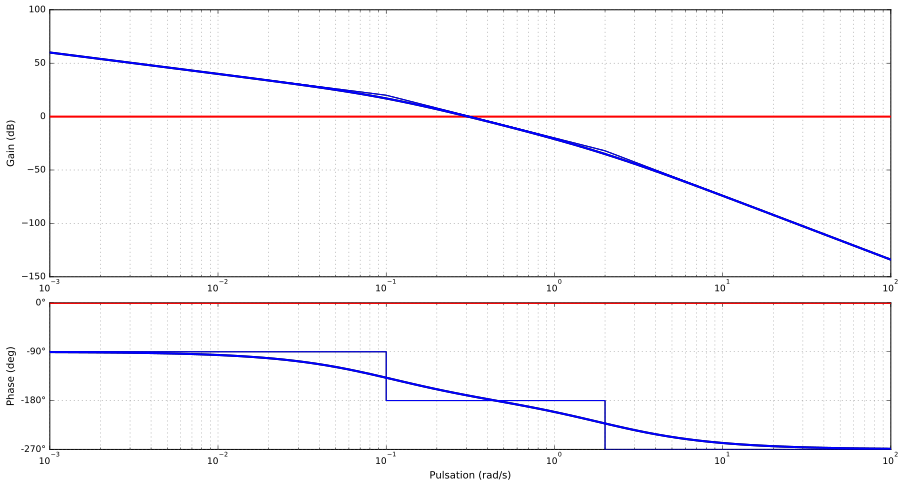
\includegraphics[width=\linewidth]{fig_03}
%\end{center}
%\end{minipage}\hfill
%\begin{minipage}[c]{.46\linewidth}
%\begin{center}
%\includegraphics[width=.9\linewidth]{fig_01}
%\end{center}
%\end{minipage}

\ifprof
\else
\fi

%
%\begin{center}
%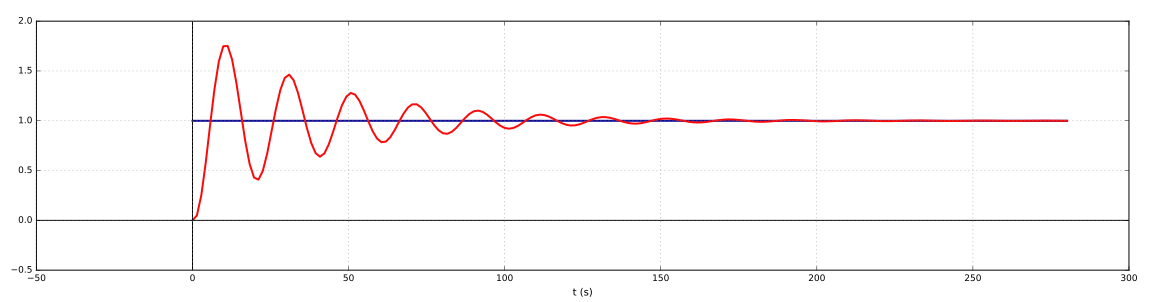
\includegraphics[width=\linewidth]{fig_02}
%\end{center}
%
%\begin{center}
%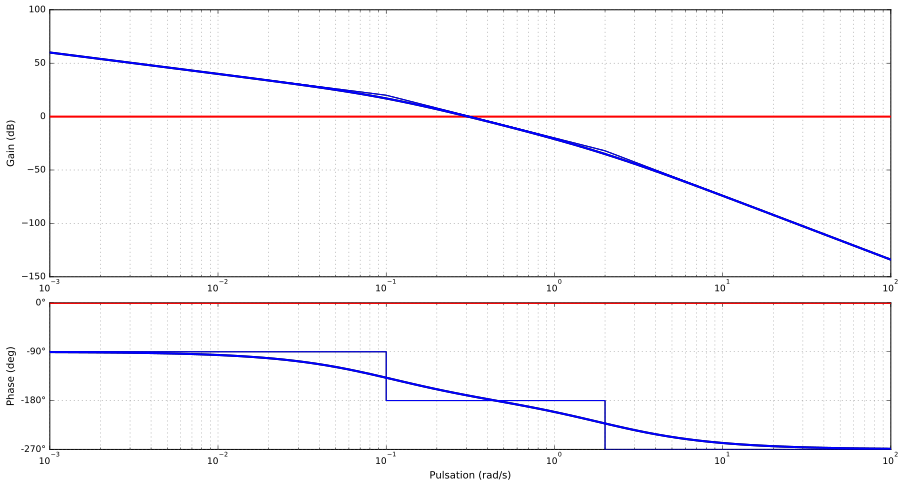
\includegraphics[width=\linewidth]{fig_03}
%\end{center}
%
%\begin{center}
%\includegraphics[width=.8\linewidth]{fig_04}
%\end{center}



%\end{document}
%
%\subsection*{Exercice 3 -- Applications du critère du Revers}
%
%\subparagraph*{}\textit{On donne ci-dessous les lieux de transferts de plusieurs FTBO. Déterminer, à l'aide du critère du Revers si les systèmes sont stables en BF.}
%\subparagraph*{}\textit{Pour les systèmes stables déterminer les marges de gain et de phase.}
%
%\end{multicols}
%
%\begin{center}
%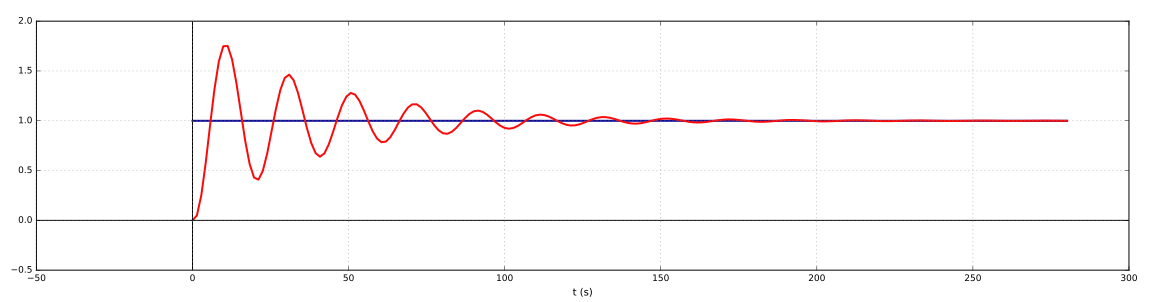
\includegraphics[width=\linewidth]{fig_02}
%\end{center}
%
%\begin{center}
%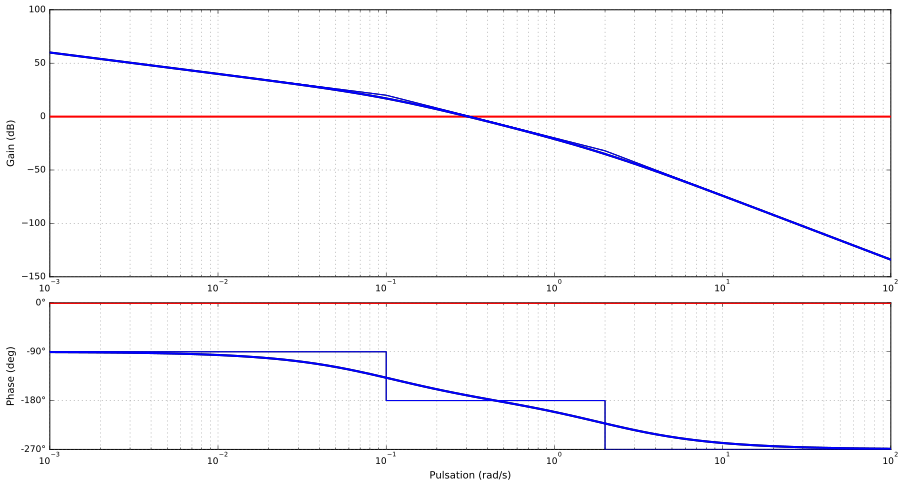
\includegraphics[width=\linewidth]{fig_03}
%\end{center}
%
%\begin{center}
%\includegraphics[width=.8\linewidth]{fig_04}
%\end{center}
%


